\documentclass[10pt,a4paper]{article}


\usepackage[utf8]{inputenc}
\usepackage{float}
\usepackage[sc]{mathpazo}
\usepackage[top=2.2cm,bottom=2.2cm,left=2.2cm,right=2.2cm]{geometry}
\usepackage{microtype}
\usepackage{xcolor}
\usepackage{graphicx}
\usepackage{booktabs}
\usepackage{tabularx}
\usepackage{array}
\usepackage{enumitem}
\usepackage{caption}
\usepackage{amsmath}
\usepackage{fancyhdr}
\usepackage{tikz}
\usetikzlibrary{arrows.meta,positioning,fit,backgrounds,calc}
\usepackage[hidelinks]{hyperref}
\urlstyle{same}
\Urlmuskip=0mu plus 2mu
\def\UrlBreaks{\do\/\do-\do.\do=\do?\do\&\do\_\do a\do b\do c\do d\do e\do f\do g\do h\do i\do j\do k\do l\do m\do n\do o\do p\do q\do r\do s\do t\do u\do v\do w\do x\do y\do z}

\captionsetup{font=small,labelfont=bf,skip=4pt}
\setlist{itemsep=1pt,topsep=3pt,parsep=0pt,leftmargin=1.4em}
\setlength{\parindent}{1.2em}
\setlength{\parskip}{2pt}
\linespread{1.06}
\emergencystretch=2em
\renewcommand{\arraystretch}{1.12}

\pagestyle{fancy}
\fancyhf{}
\fancyhead[L]{\small IT457 -- Cloud Computing}
\fancyhead[R]{\small Freshworks on AWS: Week-2 Report}
\fancyfoot[C]{\small\thepage}
\renewcommand{\headrulewidth}{0.3pt}

\newcolumntype{Y}{>{\raggedright\arraybackslash}X}
\newcommand{\code}[1]{\texttt{#1}}

\begin{document}

% ------------------------------------------------------------------ title
\begin{center}
{\small Dhirubhai Ambani University (formerly DA-IICT)\quad$|$\quad IT457 -- Cloud Computing\quad$|$\quad Autumn 2026}\\[6pt]
{\LARGE\bfseries Freshworks on AWS}\\[2pt]
{\large\bfseries From a Rails monolith to a Serverless Developer Platform}\\[3pt]
{\normalsize Week-2 Report: Case Analysis and Exercise Plan}\\[2pt]
{\small Theme-4 : Serverless and Startups}\\[2pt]
{\normalsize \textbf{Group-15} : Hriday Asnani(202301282), Jayaditya Shah (202301254), Maharshi Patel(202301486)}
\end{center}
\vspace{-4pt}
\hrule
\vspace{6pt}

\begin{abstract}
\noindent This report analyses how Freshworks, a SaaS company that started in Chennai in 2010, runs and scales on AWS, and uses that analysis to plan our hands-on exercise. We read the company's engineering posts, two AWS case studies, SEC filings and recent earnings material. Most of Freshworks' main product is a conventional Rails application on load balancers and managed databases, and its problems are mostly about protecting shared capacity from slow requests and noisy tenants. Serverless appears in one specific place: the Neo developer platform, where every marketplace app runs as an AWS Lambda function. We therefore build a small serverless proof of concept (API Gateway, Lambda, DynamoDB) in the \texttt{ap-south-1} region and measure cold starts, warm latency and cost per 1{,}000 requests. The report also gives the architecture diagrams, the problem--solution analysis, the experiment design and the division of work between the three of us.
\end{abstract}

% ------------------------------------------------------------------ 1
\section{Introduction}

This is our Week-2 submission for the IT457 project. Our assigned case is Freshworks, which falls under Theme 4 (Serverless and Startups). The implementation guide for this theme instructs us for a live API that triggers a serverless function, screenshots of the architecture (API Gateway, Lambda, DynamoDB), and a spreadsheet with a graph of cold-start versus warm latency and the cost per 1{,}000 requests. We are not expected to build a smaller Freshworks. The case gives us the context that tells us what is worth building and measuring.

One thing we only understood after reading the primary sources is that Freshworks is not really a ``serverless company''. Its biggest product, Freshdesk, is a Ruby on Rails monolith that peaks at about 500K requests per minute behind AWS load balancers~\cite{kumar2020}. Serverless shows up in a narrower place: the platform that lets outside developers write apps for the Freshworks Marketplace, which runs those apps as AWS Lambda functions~\cite{awslambda}. Because of this the report covers two parts of the company. The main product architecture explains where the scaling pain came from. The Lambda-based developer platform is the part our exercise is modelled on.

\subsection{Sources and how we used them}

Table~\ref{tab:sources} lists what we actually relied on. We separate primary sources (written by Freshworks engineers, filed with the SEC, or published by AWS) from vendor and news material, which we use only for context. Vendor case studies are written to promote the vendor, so we treat their numbers more carefully than audited ones.

\begin{table}[ht]
\centering\small
\caption{Sources used in this report.}\label{tab:sources}
\begin{tabularx}{\textwidth}{@{}>{\raggedright\arraybackslash}p{0.42\textwidth} >{\raggedright\arraybackslash}p{0.17\textwidth} Y@{}}
\toprule
Source & Type & What we took from it \\
\midrule
Freshworks Eng., ``Scaling the Freshdesk web app'' (2020)~\cite{kumar2020} & Engineering blog & Request path, five causes of slow requests, MySQL event, Semian \\
``How Freshdesk uses HAProxy at scale'' (2021)~\cite{mallapu2021} & Engineering blog & Shell routing, buffer shell \\
SRE Conf 2023 talk abstract on shells~\cite{srinivasan2023} & Conference abstract & Why shells exist, shard-to-shell mapping \\
Freshworks Eng., background jobs and Freno~\cite{bgjobs} & Engineering blog & Replica lag and job throttling \\
AWS, ``Freshworks supercharges its Marketplace with Lambda''~\cite{awslambda} & AWS case study (2020) & Lambda per app, 2017 concurrency limit \\
Form 10-K FY2021 and FY2022~\cite{tenk21,tenk22} & SEC filings & Cost of revenue, gross margin, hosting cost increases \\
Q4/FY2025 earnings release and call~\cite{er25,call25} & Company filings & Revenue, ARR, margin notes \\
AWS Global Passport case study, SCA press release~\cite{gp,sca} & AWS / company & Customer count, regional expansion, AWS agreement \\
Spot case study~\cite{spot}, Redis migration post~\cite{redis19} & Vendor / engineering & Cost-saving and managed-service trade-offs \\
\bottomrule
\end{tabularx}
\end{table}

\subsection{Corrections to our Week-1 summary}

While re-reading the Week-1 report against the original documents we found several figures that we could not trace to any source. These include the 60K RPM cap per shell, a custom Kubernetes operator running Redis on EKS, the \$337.5M AWS commitment line, and the Aurora-based database description. We have left them out here. Where the two reports disagree, this one should be taken as the corrected version. For example, the Freshworks post we found describes moving Redis \emph{away} from ElastiCache to Redis Labs~\cite{redis19}, which does not fit the EKS story.

% ------------------------------------------------------------------ 2
\section{Company background}

Freshworks was founded in 2010 and began with a single help-desk product, Freshdesk. It now sells several products (Freshdesk, Freshservice, Freshsales, Freshchat and others) and is listed on NASDAQ as FRSH. AWS describes it as serving about 70{,}000 customers worldwide~\cite{gp}; an older AWS customer page quoted 56{,}000+~\cite{rdscust}, so the base has kept growing. In financial terms, revenue was \$720.4 million in 2024 and \$838.8 million in 2025, a 16\% increase, and the company reported its first full year of GAAP profitability in 2025~\cite{er25,call25}. Annual recurring revenue ended 2025 at \$907 million~\cite{call25}.

The company's relationship with AWS is long and also commercial. In January 2024 it signed a multi-year Strategic Collaboration Agreement with AWS and started selling through AWS Marketplace; the press release says more than 500 shared customers already combine Freshworks with AWS services such as Lambda, CloudWatch, EventBridge and Amazon Connect~\cite{sca}. For international growth, AWS's own case study mentions new data centres in Dubai and London to reach customers in the Middle East, Africa and the UK~\cite{gp}.

Figure~\ref{fig:timeline} places the technical milestones we found on one line. It is not to scale, and the dates are the dates of the sources, not necessarily of the underlying change.

\begin{figure}[ht]
\centering
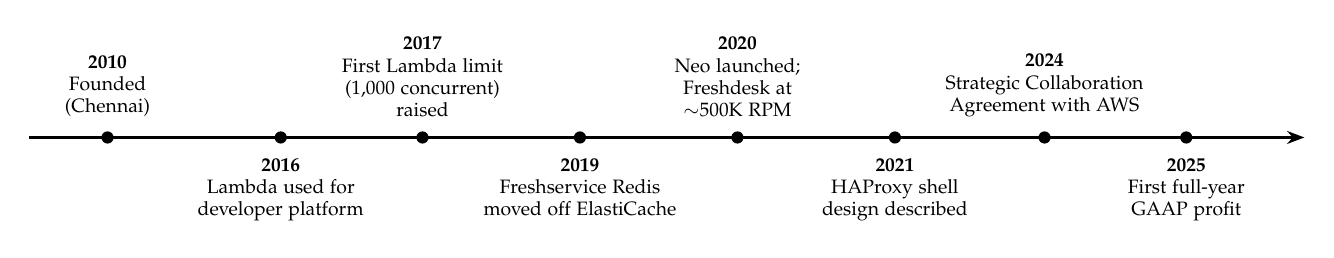
\begin{tikzpicture}[font=\scriptsize]
\draw[thick,-{Stealth[length=2.2mm]}] (0,0) -- (16.2,0);
\foreach \x/\yr/\txt/\pos in {
 1.0/2010/{Founded\\(Chennai)}/above,
 3.2/2016/{Lambda used for\\developer platform}/below,
 5.0/2017/{First Lambda limit\\(1{,}000 concurrent)\\raised}/above,
 7.0/2019/{Freshservice Redis\\moved off ElastiCache}/below,
 9.0/2020/{Neo launched;\\Freshdesk at\\$\sim$500K RPM}/above,
 11.0/2021/{HAProxy shell\\design described}/below,
 12.9/2024/{Strategic Collaboration\\Agreement with AWS}/above,
 14.7/2025/{First full-year\\GAAP profit}/below}
{
  \fill (\x,0) circle (2.2pt);
  \node[\pos=4pt,align=center] at (\x,0) {\textbf{\yr}\\\txt};
}
\end{tikzpicture}
\caption{Timeline of the Freshworks--AWS events used in this report.}\label{fig:timeline}
\end{figure}

% ------------------------------------------------------------------ 3
\section{Architecture of the Freshworks platform on AWS}

Figure~\ref{fig:arch} is our redrawing of the Freshdesk web architecture, put together from the 2020 availability post~\cite{kumar2020}, the HAProxy post~\cite{mallapu2021}, the shell talk abstract~\cite{srinivasan2023} and the background-jobs post~\cite{bgjobs}. The orange boxes are AWS managed services. We should say that these posts are from 2020 to 2023, so the current production setup may differ in details.

\begin{figure}[t]
\centering
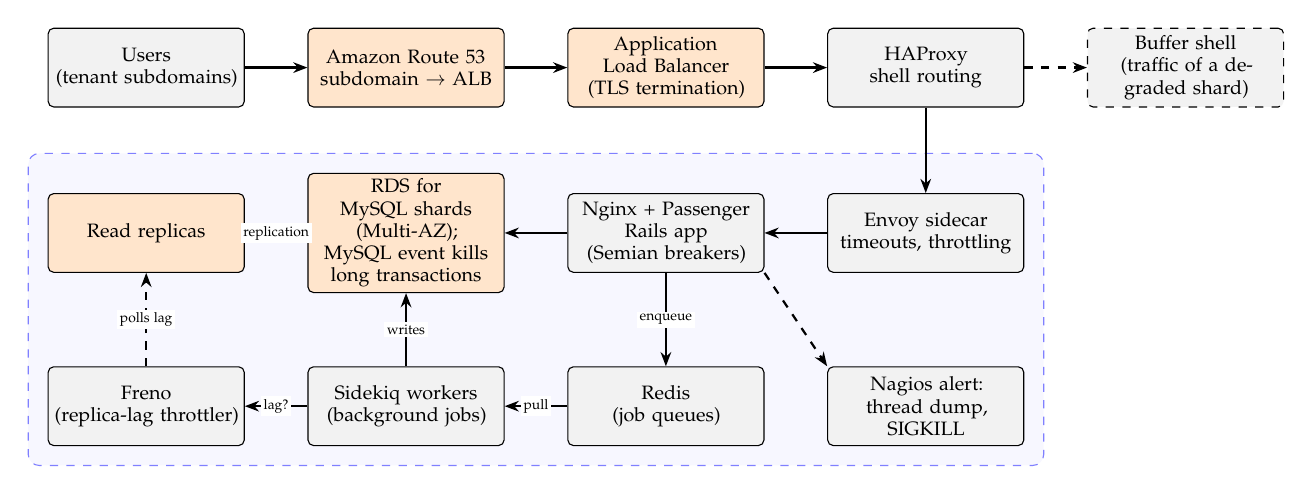
\begin{tikzpicture}[
 blk/.style={draw,rounded corners=2pt,fill=gray!10,text width=2.35cm,minimum height=1.0cm,align=center,font=\scriptsize,inner sep=2pt},
 awsb/.style={blk,fill=orange!20},
 dsh/.style={blk,dashed},
 arr/.style={-{Stealth[length=1.8mm]},thick},
 lab/.style={font=\tiny,fill=white,inner sep=1pt}]
\node[blk]  (users) at (0,0)    {Users\\(tenant subdomains)};
\node[awsb] (r53)   at (3.3,0)  {Amazon Route 53\\subdomain $\to$ ALB};
\node[awsb] (alb)   at (6.6,0)  {Application Load Balancer\\(TLS termination)};
\node[blk]  (hap)   at (9.9,0)  {HAProxy\\shell routing};
\node[dsh]  (buf)   at (13.2,0) {Buffer shell\\(traffic of a degraded shard)};
\node[blk]  (env)   at (9.9,-2.1)  {Envoy sidecar\\timeouts, throttling};
\node[blk]  (pas)   at (6.6,-2.1)  {Nginx + Passenger\\Rails app\\(Semian breakers)};
\node[awsb] (rds)   at (3.3,-2.1)  {RDS for MySQL shards\\(Multi-AZ);\\MySQL event kills\\long transactions};
\node[awsb] (rep)   at (0,-2.1)    {Read replicas};
\node[blk]  (fre)   at (0,-4.3)    {Freno\\(replica-lag throttler)};
\node[blk]  (sk)    at (3.3,-4.3)  {Sidekiq workers\\(background jobs)};
\node[blk]  (red)   at (6.6,-4.3)  {Redis\\(job queues)};
\node[blk]  (nag)   at (9.9,-4.3)  {Nagios alert:\\thread dump, SIGKILL};
\draw[arr] (users) -- (r53);
\draw[arr] (r53) -- (alb);
\draw[arr] (alb) -- (hap);
\draw[arr,dashed] (hap) -- (buf);
\draw[arr] (hap) -- (env);
\draw[arr] (env) -- (pas);
\draw[arr] (pas) -- (rds);
\draw[arr] (rds) -- node[lab]{replication} (rep);
\draw[arr] (pas) -- node[lab]{enqueue} (red);
\draw[arr] (red) -- node[lab]{pull} (sk);
\draw[arr] (sk) -- node[lab]{writes} (rds);
\draw[arr] (sk) -- node[lab]{lag?} (fre);
\draw[arr,dashed] (fre) -- node[lab]{polls lag} (rep);
\draw[arr,dashed] (pas.south east) -- (nag.north west);
\begin{scope}[on background layer]
\node[draw=blue!50,dashed,rounded corners=4pt,fill=blue!3,fit=(env)(pas)(rds)(rep)(fre)(sk)(red)(nag),inner sep=7pt] {};
\end{scope}
\end{tikzpicture}
\caption{Freshdesk web request path and background processing as described in the engineering posts. The dashed blue region is what we understand as one ``shell''.}\label{fig:arch}
\end{figure}

\paragraph{Ingress and shells.} Every tenant gets its own subdomain, for example \code{customer1.freshdesk.com}. Route~53 records for these subdomains point to one of several Application Load Balancers, which terminate TLS and forward to HAProxy instances~\cite{kumar2020}. HAProxy is where the \emph{shell} routing lives. A shell is a logical grouping of compute resources, and a set of database shards is mapped to each shell~\cite{mallapu2021,srinivasan2023}. HAProxy can choose a shell by domain, by subscription type, by shard, and by request header; migration requests, for example, carry a header that sends them to a separate shell with its own Redis endpoint for Sidekiq~\cite{mallapu2021}. If a shard is degraded, its traffic is sent to a dedicated buffer shell until it recovers. The default shell is defined in a JSON file kept in Git.

\paragraph{Inside a shell.} Requests go through an Envoy sidecar, then Nginx, then the Passenger process pool that runs the Rails code~\cite{kumar2020}. Passenger processes are single-threaded, so one process serves one request at a time. Envoy also proxies outbound calls to internal services and gives the team timeouts, rate limiting, retries and metrics for them.

\paragraph{Data and background work.} Customer data is on sharded Amazon RDS for MySQL with Multi-AZ, plus replicas~\cite{kumar2020}. Slow or non-urgent work goes to Sidekiq workers backed by Redis, and those workers check Freno before writing heavily~\cite{bgjobs}. Long-running requests trigger Nagios alerts, after which an engineer takes a thread dump and kills the stuck process, and Passenger starts a replacement~\cite{kumar2020}.

\paragraph{The developer platform.} The Neo platform and its Marketplace are the second architecture we care about, and we describe it separately in Section~\ref{sec:neo} because our exercise follows it.

% ------------------------------------------------------------------ 4
\section{The problem}

Freshworks' own engineering writing is quite direct about what hurt. We group the problems into five.

\paragraph{4.1 Slow requests eat shared capacity.} Because each Passenger process handles one request at a time and spawning new processes costs time and memory, a request that runs too long ties up a worker. The post notes that at about 500K RPM even a small change in response time makes requests queue, which users notice as a slow product~\cite{kumar2020}. It lists the usual culprits: long database transactions, an unresponsive shard, slow outbound calls to other services, spam or denial-of-service on one tenant, and bugs in application code.

\paragraph{4.2 Blast radius in a multi-tenant system.} In a multi-tenant design one customer's problem can cascade to its neighbours. The SRE Conf abstract says that there were incidents where a simple failure for one customer at the database level threatened to take down the entire web cluster~\cite{srinivasan2023}.

\paragraph{4.3 Background jobs hurting the databases.} Heavy writes from Sidekiq workers caused replication lag between the primary and its replicas, and some Sidekiq jobs caused CPU spikes on the database~\cite{bgjobs}.

\paragraph{4.4 Running other people's code.} The Marketplace lets third-party developers write apps that react to events such as ticket updates. Freshworks needed to run that code at unpredictable volume without making developers think about servers~\cite{awslambda}. This is the problem that connects most directly to our theme.

\paragraph{4.5 Hosting cost.} In the 10-K, third-party hosting costs grew by \$6.9 million in 2021 and by \$8.5 million in 2022~\cite{tenk21,tenk22}. These are small compared with revenue but they are the line the company says it manages through economies of scale (Section~\ref{sec:cost}).

% ------------------------------------------------------------------ 5
\section{The solutions}

The striking thing, to us, is that few of the fixes are ``add more servers''. Most are guardrails that stop one slow thing from spreading. Table~\ref{tab:solutions} summarises them; the paragraphs after it give the details we found most interesting.

\begin{table}[ht]
\centering\small
\caption{Problems and the mechanisms Freshworks describes for them.}\label{tab:solutions}
\begin{tabularx}{\textwidth}{@{}l Y l@{}}
\toprule
Problem & Mechanism & Source \\
\midrule
Long database transactions & Scheduled MySQL event that kills transactions older than a limit (25\,s in the sample code) & \cite{kumar2020} \\
Unresponsive shard & Semian circuit breaker in the Rails app so requests fail fast & \cite{kumar2020} \\
Slow outbound calls & Strict timeouts, HTTP circuit breaker for search, Envoy sidecar & \cite{kumar2020} \\
Spam or abuse by one tenant & Envoy throttling by domain and IP, HAProxy deny lists, in-house throttling service, Sidekiq middleware to pause a tenant's jobs & \cite{kumar2020} \\
Stuck application code & Nagios alert, thread dump, SIGKILL, Passenger respawns the process & \cite{kumar2020} \\
Blast radius & Shell architecture with HAProxy routing and a buffer shell & \cite{mallapu2021,srinivasan2023} \\
Replica lag from jobs & Freno checked by Sidekiq workers before they write & \cite{bgjobs,freno} \\
Running third-party apps & Each app deployed as an AWS Lambda function & \cite{awslambda} \\
EC2 cost for OpsWorks fleet & Spot instances via Spot Elastigroup (vendor reports 65\% saving) & \cite{spot} \\
\bottomrule
\end{tabularx}
\end{table}

\paragraph{Killing long transactions.} The team created a MySQL event that reads InnoDB's \code{INNODB\_TRX} table on a schedule and calls the RDS procedure \code{mysql.rds\_kill} for any transaction older than a threshold; the example in the post uses 25 seconds and skips a few internal users such as the migration user. The authors warn that the application and ORM must be tested against rollbacks, since older versions of Rails swallowed connection errors and left orphaned records~\cite{kumar2020}.

\paragraph{Semian.} The circuit breaker comes from Shopify. Before enabling it the team built a dry-run mode that only logs state changes, which exposed a MySQL timeout error that Semian did not capture (they sent a fix upstream) and a monitoring agent whose own connection pool was being counted as queries~\cite{kumar2020}. They are honest about the limits: Semian works best when the whole database is unreachable, such as in a Multi-AZ failover, but cannot help when a few busy tables are locked, and it works per process rather than per host. They were evaluating a ProxySQL sidecar as the next step.

\paragraph{Freno.} Freno is a throttler written at GitHub that tells cooperating clients to slow down when MySQL replication lag crosses a threshold~\cite{freno}. In Freshworks' setup, a Sidekiq worker asks Freno before starting; if there is lag, the job is put back in the queue after a delay equal to the lag or 60 seconds, whichever is higher. The team reports that this eliminated primary-to-replica lag from background jobs~\cite{bgjobs}.

\paragraph{Managed is not always the answer.} A 2019 post describes Freshservice moving its Redis from ElastiCache to Redis Labs with zero downtime, because ElastiCache did not support the \code{SLAVEOF} command the team needed to change replication on the fly~\cite{redis19}. For our project this is a useful reminder that a startup chooses services on practical grounds rather than loyalty to one provider.

% ------------------------------------------------------------------ 6
\section{Serverless in Freshworks: the Neo developer platform}\label{sec:neo}

Neo is the unified platform behind Freshworks' newer products and its Marketplace, which had over 1{,}200 apps when Neo was announced in 2020~\cite{neo}. According to the AWS case study, Freshworks built command-line tools and its own SDK around Lambda so that a developer only writes the business logic of an app as a few methods, and Freshworks packages and deploys it as a function~\cite{awslambda}. Every app published to the platform becomes a Lambda function, and when an event arrives (the case study uses a ticket update as the example) the platform finds the apps subscribed to that event and triggers their functions. Each trigger is one Lambda invocation. Figure~\ref{fig:neo} shows the flow.

\begin{figure}[ht]
\centering
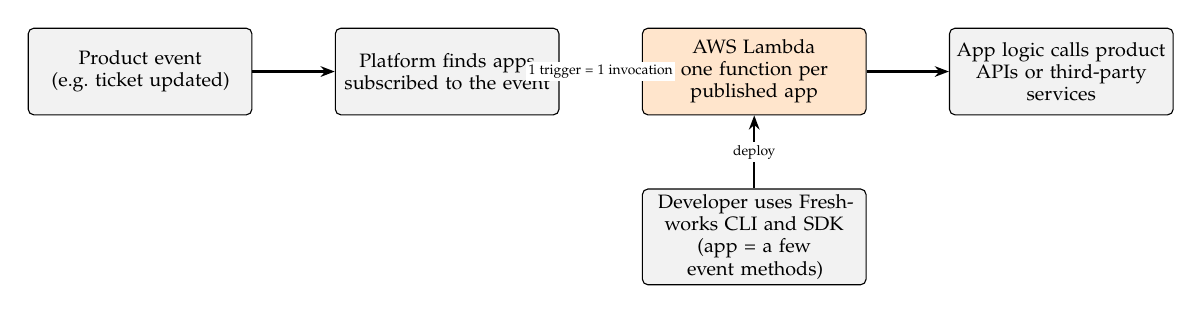
\begin{tikzpicture}[
 blk/.style={draw,rounded corners=2pt,fill=gray!10,text width=2.7cm,minimum height=1.1cm,align=center,font=\scriptsize,inner sep=2pt},
 awsb/.style={blk,fill=orange!20},
 arr/.style={-{Stealth[length=1.8mm]},thick},
 lab/.style={font=\tiny,fill=white,inner sep=1pt}]
\node[blk]  (ev)  at (0,0)    {Product event\\(e.g.\ ticket updated)};
\node[blk]  (sub) at (3.9,0)  {Platform finds apps\\subscribed to the event};
\node[awsb] (lam) at (7.8,0)  {AWS Lambda\\one function per\\published app};
\node[blk]  (ext) at (11.7,0) {App logic calls product\\APIs or third-party\\services};
\node[blk]  (dev) at (7.8,-2.1) {Developer uses Freshworks CLI and SDK\\(app = a few event methods)};
\draw[arr] (ev) -- (sub);
\draw[arr] (sub) -- node[lab]{1 trigger = 1 invocation} (lam);
\draw[arr] (lam) -- (ext);
\draw[arr] (dev) -- node[lab]{deploy} (lam);
\end{tikzpicture}
\caption{Event flow of the Freshworks developer platform, based on the AWS Lambda case study~\cite{awslambda}.}\label{fig:neo}
\end{figure}

A few details from that case study matter for us. The developer platform is the largest Lambda user among several Freshworks teams, and it runs code written by third parties, not by Freshworks engineers. An engineer quoted in the study says the team started this work in 2016 and, as traffic spiked, never hit a Lambda soft limit until 2017, when it reached 1{,}000 concurrent invocations and had the limit raised without trouble~\cite{awslambda}. A Freshworks product leader also said at the Neo launch that Lambda lets the platform handle hundreds of millions of near real-time events~\cite{neo}. Finally, the case-study listing we found also includes a vendor study about optimising Freshworks' Lambda developer platform~\cite{listing}; we could only see its title, but it suggests that tuning Lambda cost and performance becomes a real topic at that scale.

There are two reasons this part of Freshworks is a good fit for the exercise. First, the workload is event-driven and bursty, which is where per-invocation billing and automatic scaling help. Second, the two usual costs of that model, cold starts and concurrency limits, are things the company ran into or had to plan for. Freshworks has not published its Lambda memory settings, runtimes, latencies or bill, so our proof of concept is an analogue of the pattern and not a copy of their system.

% ------------------------------------------------------------------ 7
\section{Cost and outcomes}\label{sec:cost}

Freshworks does not publish an itemised AWS bill, so a full cost breakdown is not possible from public data. What we can do is collect the numbers that are public (Table~\ref{tab:cost}) and be careful about what they prove.

\begin{table}[ht]
\centering\small
\caption{Public financial and cost data points found in primary documents.}\label{tab:cost}
\begin{tabularx}{\textwidth}{@{}l Y l@{}}
\toprule
Item & Figure & Source \\
\midrule
FY2021 cost of revenue & \$78.0M; gross margin 79\% (same as 2020); third-party hosting +\$6.9M & \cite{tenk21} \\
FY2022 cost of revenue & \$95.8M (+23\%); gross margin 81\%; third-party hosting +\$8.5M & \cite{tenk22} \\
FY2024 revenue & \$720.4M & \cite{er25} \\
FY2025 revenue & \$838.8M (+16\%) & \cite{er25} \\
ARR at end of 2025 & \$907M & \cite{call25} \\
Q4 2025 non-GAAP gross margin & 86.8\%, including a \$1.5M AWS contract credit & \cite{call25} \\
OpsWorks fleet on Spot instances & 65\% cloud-cost saving (vendor-reported) & \cite{spot} \\
\bottomrule
\end{tabularx}
\end{table}

Reading these together: in 2021 hosting cost grew by \$6.9 million and the gross margin did not move, while in 2022 hosting grew by more (\$8.5 million) yet the margin went up two points. The 10-K attributes the improvement to economies of scale, mainly in third-party hosting~\cite{tenk22}. So the hosting bill grew more slowly than revenue. We also noticed that the Q4 2025 margin figure includes an AWS contract credit of \$1.5 million~\cite{call25}, which flatters that quarter a little.

We are careful not to claim more than this. Gross margin depends on many things (support staffing, payment fees, licences), so we cannot say that any one architectural change caused the margin to rise. Our Week-1 report implied that, and we have removed it. The honest summary is that the numbers are consistent with Freshworks getting more from each dollar of hosting as it grew, and that the engineering posts describe plausible mechanisms. It is also why our exercise builds its own unit-economics numbers (cost per 1{,}000 requests) instead of borrowing Freshworks'.

% ------------------------------------------------------------------ 8
\section{Exercise plan}

\subsection{Objective and hypotheses}

The exercise for Theme 4 is to build a small serverless application, make it reachable through a public API, and measure its latency and cost. We wrote down three hypotheses that we want the data to confirm or contradict, so that the results section of the final report has something definite to discuss.

\begin{enumerate}
\item[\textbf{H1.}] The first request after a Lambda environment has been idle or reconfigured (a cold start) is noticeably slower than later requests (warm), and the difference is visible both from the client and in the \code{Init Duration} reported by Lambda.
\item[\textbf{H2.}] Giving the function more memory reduces its duration, so the cost per request may stay roughly flat even though the price per millisecond rises.
\item[\textbf{H3.}] For a function this small, the per-request charges of API Gateway and DynamoDB are larger than the Lambda compute charge, so changing memory changes the total cost only slightly.
\end{enumerate}

We do not yet know whether these are true. For example, H3 could fail if our function turns out to be slower than expected.

\subsection{System to be built}

The application is deliberately tiny, as the implementation guide says. To tie it to the case, it is a ticket-intake endpoint: a client posts a support ticket and the function stores it, much like a Marketplace app reacting to a ticket event. The payload looks like this:

{\small
\begin{verbatim}
POST /tickets
{ "tenant_id": "acme", "ticket_id": "T-1042",
  "subject": "Cannot reset password", "priority": "high" }
\end{verbatim}}

The Lambda handler validates the JSON, writes one item to a DynamoDB table and returns a short JSON response with status 201. The table uses on-demand capacity, \code{tenant\_id} as partition key and \code{ticket\_id} as sort key, which echoes Freshworks' per-tenant separation. Items get a time-to-live attribute so that our test data deletes itself. A second route, \code{GET /tickets}, is only there to check that the writes worked. Figure~\ref{fig:poc} shows the architecture and the measurement pipeline around it.

\begin{figure}[ht]
\centering
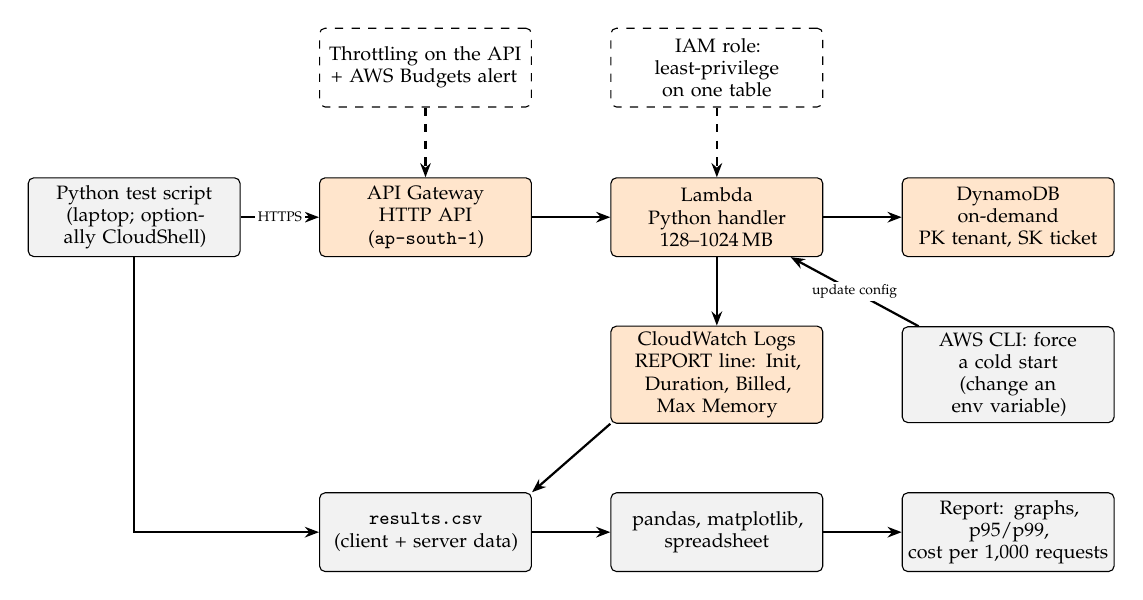
\begin{tikzpicture}[
 blk/.style={draw,rounded corners=2pt,fill=gray!10,text width=2.55cm,minimum height=1.0cm,align=center,font=\scriptsize,inner sep=2pt},
 awsb/.style={blk,fill=orange!20},
 note/.style={blk,dashed,fill=white},
 arr/.style={-{Stealth[length=1.8mm]},thick},
 lab/.style={font=\tiny,fill=white,inner sep=1pt}]
\node[blk]  (cli)  at (0,0)     {Python test script\\(laptop; optionally CloudShell)};
\node[awsb] (gw)   at (3.7,0)   {API Gateway\\HTTP API\\(\code{ap-south-1})};
\node[awsb] (lam)  at (7.4,0)   {Lambda\\Python handler\\128--1024\,MB};
\node[awsb] (ddb)  at (11.1,0)  {DynamoDB\\on-demand\\PK tenant, SK ticket};
\node[note] (bud)  at (3.7,1.9) {Throttling on the API\\+ AWS Budgets alert};
\node[note] (iam)  at (7.4,1.9) {IAM role:\\least-privilege on one table};
\node[awsb] (cw)   at (7.4,-2.0) {CloudWatch Logs\\REPORT line: Init, Duration, Billed, Max Memory};
\node[blk]  (awscli) at (11.1,-2.0) {AWS CLI: force a cold start\\(change an env variable)};
\node[blk]  (csv)  at (3.7,-4.0) {\code{results.csv}\\(client + server data)};
\node[blk]  (pd)   at (7.4,-4.0) {pandas, matplotlib,\\spreadsheet};
\node[blk]  (rep)  at (11.1,-4.0) {Report: graphs, p95/p99,\\cost per 1{,}000 requests};
\draw[arr] (cli) -- node[lab]{HTTPS} (gw);
\draw[arr] (gw) -- (lam);
\draw[arr] (lam) -- (ddb);
\draw[arr,dashed] (bud) -- (gw);
\draw[arr,dashed] (iam) -- (lam);
\draw[arr] (lam) -- (cw);
\draw[arr] (awscli) -- node[lab]{update config} (lam);
\draw[arr] (cli.south) |- (csv.west);
\draw[arr] (cw.south west) -- (csv.north east);
\draw[arr] (csv) -- (pd);
\draw[arr] (pd) -- (rep);
\end{tikzpicture}
\caption{Planned proof of concept (top) and measurement pipeline (bottom).}\label{fig:poc}
\end{figure}

\subsection{Experiments}

Table~\ref{tab:exp} lists the experiments. E1 and E2 are required to meet the deliverables. E3 and E4 are extras that we will do only if time allows, in the order listed.

\begin{table}[ht]
\centering\small
\caption{Planned experiments.}\label{tab:exp}
\begin{tabularx}{\textwidth}{@{}l Y Y Y@{}}
\toprule
ID & What varies / what we do & Samples & Output \\
\midrule
E1 & Baseline at 128\,MB: cold versus warm latency & 30 cycles, each 1 cold request followed by 100 warm & Stats table, line plot of latency by request number, box plot \\
E2 & Memory sweep: 128, 256, 512, 1024\,MB with the same cycle & 4 configurations $\times$ 30 cycles & Latency and cost versus memory \\
E3 (extra) & Same code in Python and Node.js at one memory size & 30 cycles each & Cold-start comparison by runtime \\
E4 (extra) & Burst of concurrent requests after a forced cold start (Locust or k6) & A few bursts at different concurrency & How many parallel cold starts occur \\
E5 & Cost model from measured billed duration, with and without free tier & Calculation & Cost per 1{,}000 requests and at larger volumes \\
\bottomrule
\end{tabularx}
\end{table}

\subsection{Measurement method}

A cold start will be forced by changing an environment variable on the function with the AWS CLI. This makes Lambda discard the old execution environment, so the next call must initialise a new one. After each forced cold start our script sends one request and then 100 consecutive requests, recording the time of each with a monotonic clock. To check that the forced method is representative, we will also do a few trials where we simply wait a long time without touching the function.

The client time includes our network, API Gateway and Lambda, so it is not the same as what Lambda reports. For the server side we use the \code{REPORT} line that Lambda writes to CloudWatch Logs for every invocation, which contains the duration, billed duration, memory size, maximum memory used and, for cold starts only, the initialisation duration. We will pull these with CloudWatch Logs Insights and join them to the client records. Reporting both lets us say how much of the total latency was Lambda initialisation and how much was everything else. For each group we report mean, median, minimum, maximum, p95 and p99, since averages hide the tail. All raw data goes into the repository as CSV so the graphs can be regenerated.

\subsection{Cost model}

The cost of 1{,}000 requests is the sum of three charges: API Gateway per request, Lambda (a per-request charge plus a charge per GB-second), and DynamoDB write request units. With memory $m$ in GB and average billed duration $t_b$ in seconds,
\[
C_{1000} = 1000\,\bigl(p_{\text{gw}} + p_{\text{req}} + p_{\text{gbs}}\, m\, t_b + p_{\text{ddb}}\bigr),
\]
where $p_{\text{gw}}$, $p_{\text{req}}$, $p_{\text{gbs}}$ and $p_{\text{ddb}}$ are the unit prices. We will read the unit prices for the Mumbai region from the AWS pricing pages and the AWS Pricing Calculator in Week 3, since prices change and we do not want to rely on remembered numbers. The model will be a spreadsheet with the prices and measured values as input cells, so we can change memory size and see the effect. We will compute it with and without the free tier (with it the answer is almost zero and says nothing), and then extend it to 1 million, 100 million and 1 billion requests per month, which connects back to the Freshworks scaling story. CloudWatch log storage is a small extra cost that we will note separately.

\subsection{Threats to validity}

Our measurements will have flaws that we should state openly. Home internet latency will add noise, so we will repeat runs at different times and, if possible, also run the script from AWS CloudShell in the same region. A forced cold start through a configuration change may not behave exactly like a natural idle timeout, hence the extra idle trials. The first requests to API Gateway may also have their own warm-up effect that we cannot separate from Lambda. Finally, a single small function is not the same as Freshworks' fleet, so we will not extrapolate conclusions beyond our setup.

\subsection{Mapping to the required deliverables}

\begin{table}[ht]
\centering\small
\caption{How our work maps to the Theme 4 deliverables.}\label{tab:deliv}
\begin{tabularx}{\textwidth}{@{}Y Y l@{}}
\toprule
Required by the guide & Our artefact & Lead \\
\midrule
Live API URL triggering a serverless function & API Gateway invoke URL for \code{POST /tickets}, kept live until the viva & M2 \\
Screenshots of the serverless architecture & Console views of API Gateway, Lambda, DynamoDB table and IAM role & M2 \\
Spreadsheet and graph of cold versus warm latency & \code{results.csv}, statistics sheet, plots from E1 and E2 & M3 \\
Cost per 1{,}000 requests & Cost-model spreadsheet (E5) & M3 \\
Case study report, 10 pages now and results later & This report plus the Week-3 results add-on & M1 \\
GitHub repository with regular commits & Code, scripts, raw data, README; commits from all three of us & All \\
\bottomrule
\end{tabularx}
\end{table}

% ------------------------------------------------------------------ 9
\section{Roles of team members}

With the code portion being lesser and most of the work on AWS configuration and measurement, we split the work by component so that each of us owns something crucial in the project. We also agreed that each member reviews another member's part, so no one is the only person who understands a piece.

\begin{table}[H]
\centering\small
\caption{Division of responsibilities.}\label{tab:roles}
\begin{tabularx}{\textwidth}{@{}l Y Y@{}}
\toprule
Member & Owns & Also does \\
\midrule
Hriday \& Maharshi  \newline (case study, documentation and measurement analysis) & Freshworks research and architecture diagrams, this report and its later add-ons, references, the weekly progress document, final report assembly. Measurement script, AWS CLI cold-start automation, Logs Insights queries, pandas analysis and plots, statistics and cost spreadsheets & Write the cost-model discussion with group; review the AWS setup notes. Running the extra experiments E3 and E4 if time allows; reviews the report's results section \\
Jayaditya \newline (AWS build) & DynamoDB table, IAM role, Lambda function and handler code, API Gateway route and throttling, CloudWatch access, budget alert, architecture screenshots & Optional infrastructure-as-code template; reviews the measurement script \\
\bottomrule
\end{tabularx}
\end{table}

All three of us will commit to the repository from our own components. In the repository we will keep \code{lambda/}, \code{measure/}, \code{analysis/}, \code{data/} and \code{docs/} folders, along with separate folders to mark each week's progress. Also, a README that explains how to reproduce the results. Each member will also run at least one measurement session, so that each of us can explain how the numbers were produced.

\begin{table}[ht]
\centering\small
\caption{Plan for the remaining weeks.}\label{tab:sched}
\begin{tabularx}{\textwidth}{@{}l Y@{}}
\toprule
Week & Plan \\
\midrule
Week 3 & Early: M2 creates the table, role, function and API; M3 writes the measurement script against the live URL; M1 prepares the results sections. Middle: smoke test, first E1 run, screenshots. Late: full E1 and E2 runs, analysis, cost model, results add-on to the report. \\
Week 4 & Extra experiments if time allows; finish the report; clean the repository and README; confirm the URL works from a different network; check the AWS bill. \\
Week 5 & Viva preparation with mock questions on both the case and our own build; keep the API live until the viva, then delete the resources. \\
\bottomrule
\end{tabularx}
\end{table}

% ------------------------------------------------------------------ 10
\section{Risks and conclusion}

\begin{table}[ht]
\centering\small
\caption{Main risks and what we will do about them.}\label{tab:risks}
\begin{tabularx}{\textwidth}{@{}Y Y@{}}
\toprule
Risk & Mitigation \\
\midrule
A public URL gets flooded and creates a bill & Throttling on the API, an AWS Budgets alert set on day one, and a short script to disable the route \\
Cold-start numbers are noisy & Many samples, repeat at different times, report percentiles not just averages \\
IAM or region mistakes waste time & Least-privilege role created once by M2 and reviewed by another member; everything in one region \\
Prices used in the cost model are out of date & Read from the AWS pricing pages in Week 3 and record the date \\
Only one person understands each part & Cross-review and one measurement session per member \\
\bottomrule
\end{tabularx}
\end{table}

In short, Freshworks grew from a start-up product to a global SaaS company on AWS by protecting shared capacity with many small guardrails, and by letting outside developers run code on Lambda without managing servers. The public sources do not give us Freshworks' internal Lambda numbers, so instead of repeating their claims we will measure the same kind of system ourselves. If H1 to H3 hold, we will have evidence of why the serverless pattern suits event-driven, bursty workloads and where its costs are. If they do not hold, that is also a result worth explaining in the viva.

% ------------------------------------------------------------------ refs
\begin{thebibliography}{99}\small
\setlength{\itemsep}{1pt}
\bibitem{kumar2020} Freshworks Engineering (B.~Kumar), ``Scaling the Freshdesk web app for high availability'', 15 Jul 2020. \url{https://www.freshworks.com/explore-cx/scaling-the-freshdesk-web-app-for-high-availability/}
\bibitem{mallapu2021} S.~Mallapu, ``How Freshdesk uses HAProxy at scale'', Freshworks, 24 Aug 2021. \url{https://www.freshworks.com/explore-cx/how-freshdesk-uses-haproxy-at-scale/}
\bibitem{srinivasan2023} R.~Srinivasan, ``Shell based architecture for maintaining high availability'', SRE Conf 2023 (talk submission), Sep 2023. \url{https://hasgeek.com/rootconf/sreconf-2023/sub/shell-based-architecture-for-maintaining-high-avai-PAfCRfuc4Puey7DiTUHsVs}
\bibitem{bgjobs} Freshworks Engineering, ``Behind the scenes: Safeguarding Freshdesk's infra from BG jobs''. \url{https://www.freshworks.com/saas/eng-blogs/safeguardling-freshdesk-infra-from-bg-jobs-blog/}
\bibitem{freno} GitHub, ``freno: cooperative, highly available throttler service''. \url{https://github.com/github/freno}
\bibitem{awslambda} Amazon Web Services, ``Freshworks supercharges its Marketplace with AWS Lambda'', case study, 2020. \url{https://www.aws.amazon.com/id/solutions/case-studies/freshworks}
\bibitem{neo} Freshworks, ``With CRM and Neo, Freshworks brings the iPhone moment in business software closer to reality'', 2020. \url{https://www.freshworks.com/with-crm-and-neo-freshworks-brings-the-iphone-moment-in-business-software-closer-to-reality-blog}
\bibitem{tenk21} Freshworks Inc., Form 10-K for the year ended 31 Dec 2021, SEC. \url{https://www.sec.gov/Archives/edgar/data/1544522/000162828022003537/frsh-20211231.htm}
\bibitem{tenk22} Freshworks Inc., Form 10-K for the year ended 31 Dec 2022, SEC. \url{https://www.sec.gov/Archives/edgar/data/1544522/000154452223000016/frsh-20221231.htm}
\bibitem{er25} Freshworks Inc., Earnings Release for Q4 and full year 2025. \url{https://ir.freshworks.com/files/doc_earnings/2025/q4/earnings-result/Earnings-Release-Q4-2025.pdf}
\bibitem{call25} Freshworks Q4 2025 earnings call transcript, The Motley Fool, 11 Feb 2026. \url{https://www.fool.com/earnings/call-transcripts/2026/02/11/freshworks-frsh-q4-2025-earnings-call-transcript/}
\bibitem{gp} Amazon Web Services, ``Freshworks aims for global expansion\ldots{} using AWS Global Passport'', case study. \url{https://aws.amazon.com/solutions/case-studies/freshworks-global-passport/}
\bibitem{sca} Freshworks, ``Strategic Collaboration Agreement with AWS'', press release, 29 Jan 2024. \url{https://www.tipranks.com/news/press-releases/freshworks-announces-strategic-collaboration-agreement-with-aws-to-increase-the-reach-of-its-ai-boosted-software-as-a-service}
\bibitem{rdscust} Amazon Web Services, ``Amazon RDS for MySQL customers'' (Freshworks entry). \url{https://aws.amazon.com/rds/mysql/customers/}
\bibitem{spot} Spot by NetApp, ``Freshworks case study''. \url{https://spot.io/case-study/freshworks-case-study}
\bibitem{redis19} A.~Arvind, ``Migrating Redis from ElastiCache with zero downtime'', Freshworks Engineering Blog, 27 Sep 2019. \url{https://medium.com/freshworks-engineering-blog/migrating-redis-from-elasticache-with-zero-downtime-7aeb278aa75b}
\bibitem{listing} CaseStudies.com, list of case studies featuring Freshworks as customer. \url{https://www.casestudies.com/customer/freshworks}
\end{thebibliography}

\end{document}
